\documentclass[12pt,a4paper]{article}

\usepackage{fontawesome5}
\providecommand{\faPencilAlt}{\faIcon{pencil-alt}}

\usepackage{styles/couleurs}
\usepackage{styles/mise_en_page}
\usepackage{styles/boites}
\usepackage{styles/maths}
\usepackage{styles/figures}

\usepackage{enumitem}
\usepackage{array}
\usepackage{tabularx}
\usepackage{amsmath}
\usepackage{amssymb}
\usepackage{tikz}
\usepackage{xparse}
\usepackage{pdflscape}
\usepackage{colortbl}

\usetikzlibrary{calc,arrows.meta,positioning}

\setlist[itemize]{leftmargin=1.4em,itemsep=0.15em,topsep=0.2em}
\setlist[enumerate]{leftmargin=*,itemsep=0.22em,topsep=0.25em}

\newcommand{\lignepointillee}{\noindent\dotfill\par\vspace{0.45em}}

\newcommand{\lignesreponse}[1]{%
\begin{tcolorbox}[
enhanced,colback=white,colframe=NeutreC!40,boxrule=0.5pt,arc=1.5mm,
left=3mm,right=3mm,top=2mm,bottom=1mm,before skip=2pt,after skip=2pt]
\foreach \i in {1,...,#1}{\lignepointillee}
\end{tcolorbox}}

\newcommand{\titreseq}[1]{%
\begin{center}
{\sffamily\LARGE\bfseries\color{TitreC}Séquence 7 -- Arithmétique}\\[0.2em]
{\sffamily\large\bfseries\color{SavoirC}#1}
\end{center}}

\newcommand{\grillecent}{%
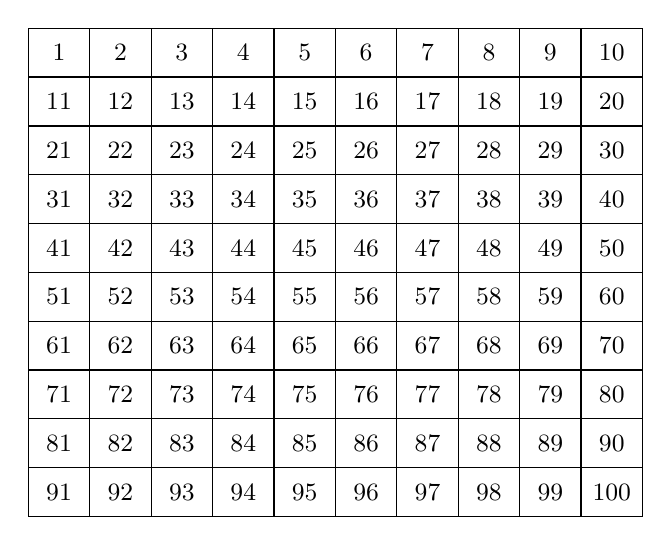
\begin{tikzpicture}[x=0.78cm,y=0.62cm]
  \foreach \n in {1,...,100}{
    \pgfmathtruncatemacro{\col}{mod(\n-1,10)}
    \pgfmathtruncatemacro{\lig}{9-floor((\n-1)/10)}
    \draw[line width=0.45pt] (\col,\lig) rectangle ++(1,1);
    \node[font=\small] at (\col+0.5,\lig+0.5) {\n};
  }
\end{tikzpicture}}

\begin{document}

\titreseq{Cours -- Divisibilité et nombres premiers}

\section{Multiples et diviseurs}

\definition{Soient \(a\) et \(b\) deux entiers, avec \(b\neq0\).

Dire que \(a\) est un \textbf{multiple} de \(b\) signifie qu'il existe
un entier \(k\) tel que :

\[
a=b\times k.
\]

On dit aussi que \(b\) est un \textbf{diviseur} de \(a\)
ou que \(a\) est \textbf{divisible par} \(b\).}

\exemple{
\[
42=6\times7.
\]

Donc \(42\) est un multiple de \(6\) et de \(7\).

Les nombres \(6\) et \(7\) sont des diviseurs de \(42\).}

\remarque{\(1\) divise tous les entiers.
Tout entier non nul est divisible par \(1\) et par lui-même.}

\subsection{Division euclidienne}

\definition{Effectuer la division euclidienne d'un entier \(a\)
par un entier non nul \(b\), c'est trouver deux entiers \(q\) et \(r\) tels que :

\[
a=b\times q+r
\qquad\text{avec}\qquad
0\leq r<b.
\]

\(q\) est le quotient entier et \(r\) est le reste.}

\exemple{La division euclidienne de \(157\) par \(12\) donne :

\[
157=12\times13+1.
\]}

\propriete{\(b\) divise \(a\) si et seulement si le reste de la division
euclidienne de \(a\) par \(b\) est nul.}

\section{Critères de divisibilité}

\renewcommand{\arraystretch}{1.45}
\begin{tabularx}{\textwidth}{
|>{\centering\arraybackslash}p{2.1cm}
|>{\raggedright\arraybackslash}X|}
\hline
\textbf{Diviseur} & \textbf{Critère}\\
\hline
\(2\) & Le chiffre des unités est \(0\), \(2\), \(4\), \(6\) ou \(8\).\\
\hline
\(3\) & La somme des chiffres est divisible par \(3\).\\
\hline
\(5\) & Le chiffre des unités est \(0\) ou \(5\).\\
\hline
\(9\) & La somme des chiffres est divisible par \(9\).\\
\hline
\(10\) & Le chiffre des unités est \(0\).\\
\hline
\end{tabularx}

\exemple{Pour \(4\,590\) :

\begin{itemize}
  \item il est divisible par \(2\), car son chiffre des unités est \(0\) ;
  \item il est divisible par \(5\) et par \(10\), car il se termine par \(0\) ;
  \item \(4+5+9+0=18\), donc il est divisible par \(3\) et par \(9\).
\end{itemize}}

\section{Nombres premiers}

\definition{Un \textbf{nombre premier} est un entier qui possède exactement
deux diviseurs différents : \(1\) et lui-même.}

\exemple{\(7\) est premier, car ses seuls diviseurs sont \(1\) et \(7\).

\(15\) n'est pas premier, car :

\[
15=3\times5.
\]

Il possède donc d'autres diviseurs que \(1\) et \(15\).}

\remarque{\(1\) n'est pas premier, car il ne possède qu'un seul diviseur.

Le seul nombre premier pair est \(2\).}

\subsection{Nombres premiers inférieurs à \(100\)}

\[
\begin{aligned}
&2,\ 3,\ 5,\ 7,\ 11,\ 13,\ 17,\ 19,\ 23,\ 29,\\
&31,\ 37,\ 41,\ 43,\ 47,\ 53,\ 59,\ 61,\ 67,\ 71,\\
&73,\ 79,\ 83,\ 89,\ 97.
\end{aligned}
\]

\methode{Pour montrer qu'un entier n'est pas premier,
il suffit de trouver un diviseur différent de \(1\) et de lui-même.

Le crible d'Ératosthène permet de construire la liste des nombres premiers
en éliminant successivement les multiples des nombres déjà repérés.}

\section{Décomposer en produit de facteurs premiers}

\definition{Décomposer un entier en produit de facteurs premiers,
c'est l'écrire comme un produit ne contenant que des nombres premiers.}

\methode{
\begin{enumerate}[label=\textbf{\arabic*.}]
  \item chercher un petit diviseur premier, à l'aide des critères ;
  \item écrire le nombre comme un produit ;
  \item poursuivre la décomposition de chaque facteur non premier ;
  \item ranger les facteurs premiers dans l'ordre croissant ;
  \item vérifier en effectuant le produit.
\end{enumerate}}

\exemple{
\[
84=12\times7
\]

\[
84=3\times4\times7
\]

\[
\boxed{84=2\times2\times3\times7}.
\]}

\remarque{Des arbres différents peuvent être utilisés,
mais ils conduisent aux mêmes facteurs premiers,
éventuellement écrits dans un ordre différent.}

\section{Utiliser les facteurs premiers avec les fractions}

\propriete{On obtient une fraction égale en multipliant
ou en divisant son numérateur et son dénominateur
par un même nombre non nul.}

\methode{Pour simplifier une fraction avec les facteurs premiers :

\begin{enumerate}[label=\textbf{\arabic*.}]
  \item décomposer le numérateur et le dénominateur ;
  \item repérer les facteurs communs ;
  \item diviser le numérateur et le dénominateur
        par le produit de ces facteurs communs.
\end{enumerate}}

\exemple{
\[
\frac{84}{126}
=
\frac{2\times2\times3\times7}
     {2\times3\times3\times7}.
\]

Le numérateur et le dénominateur possèdent les facteurs communs
\(2\), \(3\) et \(7\). On les divise donc par \(2\times3\times7=42\) :

\[
\frac{84}{126}
=
\frac{2}{3}.
\]}

\remarque{En 4e, on apprend à simplifier une fraction au maximum
à l'aide des facteurs premiers. La terminologie plus formelle
de fraction irréductible sera reprise en 3e.}

\section{Problèmes de groupes identiques}

\methode{Lorsque plusieurs quantités doivent être réparties
en groupes tous identiques, sans reste :

\begin{enumerate}[label=\textbf{\arabic*.}]
  \item le nombre de groupes doit diviser chacune des quantités ;
  \item on cherche donc leurs diviseurs communs ;
  \item si la question demande toutes les possibilités,
        on doit donner tous les diviseurs communs ;
  \item on calcule ensuite la composition de chaque groupe.
\end{enumerate}}

\exemple{Pour répartir \(36\) objets rouges et \(48\) objets bleus
en \(6\) groupes :

\[
36\div6=6
\qquad\text{et}\qquad
48\div6=8.
\]

Chaque groupe contient \(6\) objets rouges et \(8\) objets bleus.}

\aretenir{
\begin{itemize}
  \item \(a\) est un multiple de \(b\) lorsque \(a=b\times k\).
  \item Un nombre premier possède exactement deux diviseurs.
  \item Tout entier supérieur à \(1\) peut être décomposé
        en produit de facteurs premiers.
  \item Les facteurs premiers permettent de simplifier des fractions
        et de chercher des diviseurs communs.
\end{itemize}}

\end{document}
